% !TEX TS-program = XeLaTeX
% use the following command: 
% all document files must be coded in UTF-8
\documentclass[spanish]{textolivre}
% See more information on the repository: https://github.com/leolca/textolivre

% Metadata
\begin{filecontents*}[overwrite]{article.xmpdata}
    \Title{El tema de la donación de órganos en Facebook: análisis de la fanpage del INDOT de Ecuador}
    \Author{Gabriel Cevallos \sep Configurações
Jonathan Bladimir Zhiminaicela Cabrera \sep María Fernanda Fernández Gonzales \sep Sueny Paloma dos Santos}
    \Language{es-ES}
    \Keywords{donación \sep órganos \sep Facebook \sep INDOT \sep Ecuador \sep Iramuteq \sep Reinert}
    \Journaltitle{Texto Livre}
    \Journalnumber{1983-3652}
    \Volume{14}
    \Issue{3}
    \Firstpage{1}
    \Lastpage{13}
    \Doi{10.35699/1983-3652.2021.29687}

    \setRGBcolorprofile{sRGB_IEC61966-2-1_black_scaled.icc}
            {sRGB_IEC61966-2-1_black_scaled}
            {sRGB IEC61966 v2.1 with black scaling}
            {http://www.color.org}
\end{filecontents*}

\journalname{Texto Livre}
\thevolume{14}
\thenumber{3}
\theyear{2021}
\receiveddate{\DTMdisplaydate{2021}{2}{28}{-1}} % YYYY MM DD
\accepteddate{\DTMdisplaydate{2021}{4}{9}{-1}}
\publisheddate{\DTMdisplaydate{2021}{7}{30}{-1}}
% Corresponding author
\corrauthor{Gabriel Francisco Cevallos Martínez}
% DOI
\articledoi{10.35699/1983-3652.2021.29687}
%\articleid{NNNN} % if the article ID is not the last 5 numbers of its DOI, provide it using \articleid{} commmand
% Abbreviated author list for the running footer
\runningauthor{Cevallos et al}
\sectioneditorname{Daniervelin Pereira}
\layouteditorname{Anna Izabella M. Pereira}


\title{El tema de la donación de órganos en Facebook: análisis de la fanpage del INDOT de Ecuador}
\othertitle{A questão da doação de órgãos no Facebook: análise da fanpage do INDOT do Equador}
\othertitle{The issue of organ donation on Facebook: analysis of the Ecuadorian INDOT fanpage}
% if there is a third language title, add here:
%\othertitle{Artikelvorlage zur Einreichung beim Texto Livre Journal}

\author[1]{Gabriel Francisco Cevallos Martínez~\orcid{0000-0002-3115-1544}~\thanks{Email: \url{gabriel.cevallos@iaen.edu.ec}}}
\author[2]{Jonathan Bladimir Zhiminaicela Cabrera~\orcid{0000-0001-9462-9608}~\thanks{Email: \url{Jzhiminai1@utmachala.edu.ec}}}
\author[3]{María Fernanda Fernández Gonzales~\orcid{0000-0001-5220-0029}~\thanks{Email: \url{mfernandezg@est.ups.edu.ec}}}
\author[4]{Sueny Paloma dos Santos~\orcid{0000-0002-8424-893X}~\thanks{Email: \url{Slima957@puce.edu.ec}}}

\affil[1]{Instituto de Altos Estudios Nacionales, Quito, Pichincha, Ecuador.}
\affil[2]{Universidad Técnica de Machala, Machala, El Oro, Ecuador.}
\affil[3]{Universidad Politécnica Salesiana, Quito, Pichincha, Ecuador.}
\affil[4]{Pontificia Universidad Católica del Ecuador, Quito, Pichincha, Ecuador.}

\addbibresource{article.bib}
% use biber instead of bibtex
% $ biber tl-article-template

%% for spanish, use:
%%\setdefaultlanguage{spanish}
%\gappto\captionsspanish{\renewcommand{\tablename}{Tabla}} % use 'Tabla' instead of 'Cuadro'
%\AfterEndPreamble{\crefname{table}{tabla}{tablas}\Crefname{table}{Tabla}{Tablas}}

% for languages that use special fonts, you must provide the typeface that will be used
% \setotherlanguage{arabic}
% \newfontfamily\arabicfont[Script=Arabic]{Amiri}
% \newfontfamily\arabicfontsf[Script=Arabic]{Amiri}
% \newfontfamily\arabicfonttt[Script=Arabic]{Amiri}
%
% in the article, to add arabic text use: \textlang{arabic}{ ... }

% to use emoticons in your manuscript
% https://stackoverflow.com/questions/190145/how-to-insert-emoticons-in-latex/57076064
% using font Symbola, which has full support
% the font may be downloaded at:
% https://dn-works.com/ufas/
% add to preamble:
% \newfontfamily\Symbola{Symbola}
% in the text use:
% {\Symbola }

% reference itens in a descriptive list using their labels instead of numbers
% insert the code below in the preambule:
\makeatletter
\let\orgdescriptionlabel\descriptionlabel
\renewcommand*{\descriptionlabel}[1]{%
  \let\orglabel\label
  \let\label\@gobble
  \phantomsection
  \edef\@currentlabel{#1\unskip}%
  \let\label\orglabel
  \orgdescriptionlabel{#1}%
}
\makeatother
%
% in your document, use as illustraded here:
%\begin{description}
%  \item[first\label{itm1}] this is only an example;
%  % ...  add more items
%\end{description}
 

% custom epigraph - BEGIN 
%%% https://tex.stackexchange.com/questions/193178/specific-epigraph-style
\usepackage{epigraph}
\renewcommand\textflush{flushright}
\makeatletter
\newlength\epitextskip
\pretocmd{\@epitext}{\em}{}{}
\apptocmd{\@epitext}{\em}{}{}
\patchcmd{\epigraph}{\@epitext{#1}\\}{\@epitext{#1}\\[\epitextskip]}{}{}
\makeatother
\setlength\epigraphrule{0pt}
\setlength\epitextskip{0.5ex}
\setlength\epigraphwidth{.7\textwidth}
% custom epigraph - END


% if you use multirows in a table, include the multirow package
\usepackage{multirow}

% add line numbers for submission
%\usepackage{lineno}
%\linenumbers

\begin{document}
\maketitle

\begin{polyabstract}
\begin{abstract}
Este artículo analiza las interacciones de la \emph{fanpage} de Facebook del Instituto Nacional de Donación y Trasplante de Órganos, Tejidos y Células (INDOT) del Ecuador, para observar el tema de la donación como objeto de diálogo en sectores de la ciudadanía ecuatoriana. Se optó por dos análisis: primero, considerar métricas de la \emph{fanpage} como seguidores, reacciones, compartidas, registro de visitas, número de administradores y evaluaciones; segundo, un análisis lexicométrico aplicado a los textos de publicaciones, comentarios recibidos y descripciones de las imágenes. El Análisis de Reinert fue ejecutado con Iramuteq como mecanismo de precategorización y después interpretado por los investigadores. Ambos análisis se aplicaron a una matriz de datos recopilados entre el año 2012 y junio del 2020 creada de forma manual. Los resultados mostraron que la \emph{fanpage} tiene una visibilidad aceptable para la población ecuatoriana y buena evaluación. Sin embargo, no se refleja un diálogo significativo, lo que concuerda con una experiencia previa de Twitter que mostró que la donación de órganos en Ecuador tiene visibilidad nula, incluso cuando todo ciudadano es donante por ley a menos que señale lo contrario. El análisis de Reinert reveló como categorías principales la concienciación por la donación, el énfasis en la misión del instituto y los casos exitosos de trasplante, estos últimos que generan mayor diálogo reflejado en comentarios de apoyo y solicitud de ayuda. Se evidencia una amplia potencialidad de este espacio como difusor de la donación -lo cual se corresponde con experiencias de otros países- y para rendición de cuentas.  

\keywords{Donación de órganos \sep Facebook \sep INDOT \sep Ecuador \sep Iramuteq}
\end{abstract}

\begin{portuguese}
\begin{abstract}
Este artigo analisa as interações da fanpage Facebook do Instituto Nacional de Doação e Transplante de Órgãos, Tecidos e Células (INDOT) do Equador, a fim de observar o tema da doação como objeto de diálogo em setores da cidadania equatoriana. Duas análises foram escolhidas: primeiro, para considerar métricas de fanpage como seguidores, reações, ações, visitas, número de administradores e avaliações; segundo, uma análise lexicométrica aplicada aos textos das publicações, comentários recebidos e descrições das imagens. A Análise Reinert foi executada com o Iramuteq como um mecanismo de pré-categorização e depois interpretada pelos pesquisadores. Ambas as análises foram aplicadas a uma matriz criada manualmente de dados coletados entre 2012 e junho de 2020. Os resultados mostraram que a fanpage tem uma visibilidade aceitável para a população equatoriana e uma boa avaliação. Entretanto, ele não reflete um diálogo significativo, o que é consistente com uma experiência anterior no Twitter que mostrou que a doação de órgãos no Equador tem visibilidade zero, mesmo quando cada cidadão é doador por lei, a menos que de outra forma indicado. A análise de Reinert revelou como principais categorias a consciência da doação, ênfase na missão do instituto e casos de transplante bem sucedidos, estes últimos gerando um maior diálogo refletido em comentários de apoio e pedidos de ajuda. Há evidências de um amplo potencial deste espaço como disseminador de doações - o que corresponde a experiências em outros países - e de prestação de contas.  

\keywords{Doação de órgãos \sep Facebook \sep INDOT \sep Equador \sep Iramuteq}
\end{abstract}
\end{portuguese}

\begin{english}
\begin{abstract}
This article analyzes the interactions of the Facebook fanpage of the National Institute of Donation and Transplantation of Organs, Tissues and Cells (Indot) of Ecuador, to observe the donation as an object of dialogue in sectors of the Ecuadorian citizenship. Two analyzes were chosen: first, use of fanpage metrics such as followers, reactions, shares and others; and second, a lexicometric analysis applied to the texts of publications, comments, and descriptions of the images, the Reinert Analysis was executed with Iramuteq (R´s interface) as a precategorization mechanism, later interpreted by the researchers. Both analyzes were applied to a data matrix created manually between 2012 and June 2020. The results showed that the fanpage has an acceptable visibility for the Ecuadorian population and a good evaluation; on the other hand, a meaningful dialogue is not reflected, which corresponds to a previous Twitter experience that showed that organ donation in Ecuador has zero visibility, even when every citizen is a donor by law unless otherwise indicated. Reinert's analysis revealed donation awareness, emphasis on the Institute's mission, and successful transplant cases as main categories, the last one generating more dialogue reflected in supportive comments and requests for help. A wide potentiality of this space is evidenced as a diffuser of donations -which corresponds to the experiences of other countries- and for transparency.

\keywords{Organ donation \sep Facebook \sep INDOT \sep Ecuador \sep Iramuteq}
\end{abstract}
\end{english}

% if there is another abstract, insert it here using the same scheme
\end{polyabstract}


\section{Introducción}\label{sec-intro}
Con la entrada de las Tecnologías de la Información y la Comunicación (TICs) los espacios de intercambio y diálogo de las personas han venido transformándose y creciendo exponencialmente gracias a la digitalización permanente de la información y la convergencia de los medios \cite{maldonado2019}. Las ágoras que agrupaban a los ciudadanos para intercambiar sus posiciones, tienen ahora forma digital que las separa de lo espacial y temporal y se diversifican en función de las intencionalidades de las personas. Internet, el “tejido de nuestra sociedad” \cite{castells2002}, ha permitido que traslademos nuestros deseos, preferencias y creaciones al ciberespacio, en donde los intereses individuales adquieren visibilidad en cuanto tengan eco en lo colectivo.

Los espacios digitales, y en especial las plataformas de redes sociales agrupan millones de interacciones, generando un diluvio infinito de información \cite{levy2010} que contiene, entre otras muchas expresiones, las expectativas ciudadanas alrededor de la política pública. Es preciso comprender a las plataformas digitales como potenciales espacios de empoderamiento ciudadano que fortalezcan nuestras democracias altamente volátiles \cite{mallen2013}. 

Lo anterior no es ajeno a los Estados, los cuales trabajan en diversas estrategias vinculadas al gobierno abierto para generar medios de información y posterior diálogo entre el Estado y la ciudadanía promoviendo la transparencia y la evaluación permanente. Las instituciones en general tienen presencia en las plataformas de redes sociales, siendo las cuentas oficiales medios de difusión de las actividades institucionales, espacios para rendición de cuentas y potenciales articuladores Estado-Ciudadano alrededor de problemáticas específicas, como lo es el tema de la salud pública, muchas veces limitado por fallas en la comunicación y educación.

Los avances en las ciencias de la salud han permitido que la mayoría de la población mundial se mantenga en crecimiento y sus esperanzas de vida sean cada vez mayores. Según la Organización Mundial de la Salud, el Ecuador, a 2016, tenía más de 16 millones de habitantes y la esperanza de vida de hombres y mujeres correspondía a 74 y 79 años respectivamente. El crecimiento poblacional genera nuevos desafíos en todas las áreas, y aunque el avance tecnológico y científico sea innegable, no dejan de existir escenarios en los cuáles las expectativas de vida de un individuo dependen directamente de una terapia o intervención específica, lo que corresponde efectivamente al trasplante de órganos, acción cada vez más común en diversos escenarios, entre los que se incluyen la superación de enfermedades crónicas en etapas terminales \cite{godt, optn, unos2017}. 

El trasplante de órganos es una forma terapéutica para el tratamiento de enfermedades crónicas, de miles de personas a nivel mundial. Siendo la única opción terapéutica para quienes padecen enfermedades terminales \cite{pedroza2019}. El desarrollo técnico y científico ha permitido, el desarrollo de tecnologías como ventilación mecánica, terapia inmunosupresora, antimicrobiana, reanimación cardiopulmonar y preservación de órganos, todos aquellos avances han aumentado exponencialmente la tasa de trasplantes \cite{pedroza2019}. 

En el Ecuador, INDOT es la entidad adscrita al Ministerio de Salud Pública, encargada de la regulación y coordinación de la actividad trasplantología del Ecuador \cite{indot2011}. Dicha institución tiene como una de sus dimensiones el contacto permanente con la ciudadanía, tanto en lo referente al registro de los donantes, como en la gestión de los receptores en espera de un trasplante como nueva oportunidad de vida. A partir del 2011 se emitió una normativa específica vinculada al trasplante, denominada Ley Orgánica de Donación y Trasplante de Órganos, Tejidos y Células que tiene como propósito regular, impulsar, y entre otras, promocionar la donación de órganos bajo normas y disposiciones legales ya establecidas, en beneficio de la colectividad. Uno de los principales aspectos de dicha ley establece la disposición de hacer de cada ecuatoriano y residentes legales donantes por defecto, es decir, todos son donantes a no ser que se exprese lo contrario en las oficinas del Registro Civil del Ecuador \cite{indot2011}. 

De todas formas, la relevancia de esta normativa que apunta al bienestar general al garantizar una importante terapia de salud no parece estar debidamente ubicada en el debate colectivo, lo cual se puede verificar tanto en el hecho de que el Ecuador tiene una amplia lista de pacientes en listas de espera y también en investigaciones previas que muestran el bajo nivel de intercambio y reacciones sobre el tema en redes \cite{dos_santos2020}. 

Como una vía adecuada de comunicación el INDOT posee cuentas en diversas plataformas de redes sociales, incluidas Twitter y Facebook. En cuanto a Twitter, según \textcite{dos_santos2020} la donación en el Ecuador es un tema invisibilizado. Los investigadores realizaron un seguimiento en esa plataforma, intentando captar muestras de tweets que hicieron referencia a la donación. Para el efecto utilizaron palabras clave y hashtags específicos, incluidos varios propuestos por el INDOT como \emph{\#indotacredita} e \emph{\#indotecuador}. Los resultados mostraron que dentro de aquella plataforma el diálogo generado alrededor de la donación y sus actores es prácticamente nulo, sin que ninguno de los mensajes encontrados genere dinámicas dialógicas.

En cuanto a Facebook ha mostrado su capacidad como herramienta para movilizar a la ciudadanía alrededor de la donación, hablándose incluso de un “Efecto Facebook” referido a como campañas en esa red conseguían aumentos sustanciales de donantes en países como México, Canadá \cite{shots2012} y Estados Unidos, incluso en escenarios en donde el registro de donantes decrecía de manera constante. El análisis realizado por \textcite{cameronetal2013} sobre una campaña que consistía en que las personas puedan compartir su estado como “Donadores” mostró el incremento en un solo día de 21\% del registro promedio de donantes, así, al primer día de la iniciativa, 13.054 personas eran nuevos donantes registrados.

Las experiencias anteriores impulsaron el uso de la citada herramienta en otros países, llegando a ser 15 en el 2017. Según \textcite{cameron2015} esta red social demostró tener un mejor desempeño al captar y gestionar donantes en relación con el Sistema Oficial de EEUU, el Motor Vehicle Administration (MVA), principalmente porque el cambio del espacio formal a la red de amistades que expresan su compromiso, promueve la voluntad de cada individuo por registrarse como donador. 

Con estos antecedentes, el presente artículo tiene la intención de analizar las actuales interacciones que ocurren dentro de la \emph{fanpage} de Facebook del INDOT, estableciéndose las particularidades de las expresiones ciudadanas, para observar como la donación y el propio instituto son tratados como objeto de diálogo. Lo encontrado será útil para mejorar las formas de interacción, establecer inquietudes frecuentes y sobre todo elevar las posibilidades de difusión y discusión de la donación de órganos en el Ecuador, tema casi olvidado excepto por los directamente involucrados.


\section{Metodología}\label{sec-metodologia}
Este trabajo se vincula de manera directa con el estudio exploratorio ya citado, realizado sobre la plataforma Twitter, considerando que los programas de concienciación y apoyo a los trasplantes se promocionan cada vez más a través de estos medios \cite{henderson2017}. Aquella investigación, se enfocó en Twitter debido a la naturaleza cercana de esa plataforma con la opinión y la política pública. Sin embargo, los resultados reportaron que la donación de órganos mostraba poca visibilidad en la plataforma \cite{dos_santos2020}.

Comprendiendo la naturaleza exploratoria de esa experiencia y la siempre parcial posibilidad de captar los datos, se consideró necesario investigar el tema dentro de otra plataforma \cite{elcomercio2020}, considerando las características específicas del nuevo espacio, que posibilite acceder a más expresiones ciudadanas, para entender mejor cómo esta política es comprendida en sectores de la población y establecer algunos elementos que configuren participación ciudadana alrededor de la donación y el trasplante. 

Se considera que, a la vez que se establecen mecanismos institucionales que tienen un carácter sistemático y protocolario regidos por diferentes instancias públicas, es importante también que estas se acerquen a los espacios cotidianos de la sociedad, entre los cuales las redes sociales tienen un puesto prioritario, de esta forma la voz del ciudadano es captada tanto en los canales institucionales, así como en contextos más abiertos con otros matices que permiten entender mejor cómo la política pública ocurre en lo cotidiano. Así, la fanpage de Facebook del INDOT fue seleccionada como espacio de estudio, siendo esa plataforma la más utilizada en el país, a través de la cual se conectan un 55,4\% de ecuatorianos con internet \cite{elcomercio2020}. 

El análisis de dicha página permitió abordar desde otra perspectiva cómo la donación de órganos es percibida en el Ecuador por la ciudadanía, recuperando las interacciones provocadas por las publicaciones del instituto. Para el efecto, se combinaron análisis cuantitativos y cualitativos aplicados a datos recopilados de manera manual, sistematizados en una matriz única con los posteos de la fanpage desde su primera publicación en el año 2012 hasta junio de 2020.

El análisis cuantitativo, comprende algunos indicadores de actividad como el número de publicaciones por día y el promedio de comentarios obtenidos por publicación, lo cual permitió establecer el nivel de dinámica de la página. Para el efecto, dentro de la matriz se registró por cada publicación los siguientes datos: fecha, hora, número de reacciones por tipo, número de compartidas, presencia de imágenes, enlaces y los textos correspondientes a la descripción de la publicación y los comentarios recibidos.

En cuanto al análisis cualitativo, se consideraron tres grupos de textos: aquellos que pertenecen a las publicaciones del Indot, los comentarios ciudadanos y las descripciones que hicieron los investigadores sobre los enlaces o imágenes sin textos específicos, a esos documentos se les aplicó análisis lexicométrico apoyado en Iramuteq, un interfaz de R. 

La lexicometría tiene como premisa que en todo documento pueden identificarse estructuras tales que demuestran una presencia significativamente frecuente y combinen sujetos, verbos y complementos, de manera que el resultado obtenido adquiere forma de ideas generales presentes en el texto \cite{morales_del_rio2019}.  

El proceso de lexicometría precisa de procesamiento previo que consiste en la lematización, es decir, la agrupación de palabras similares para asignar a cada conjunto una sola representante llamada palabra raíz o forma. Por ejemplo, si el aplicativo encuentra en un texto palabras como estudiar, estudié y estudia, las agrupa y representa con el verbo correspondiente en infinitivo, en este caso “estudiar” \cite[p. 9]{ruiz_bueno2016}. Es  en el texto lematizado donde se aplican procedimientos léxicos métricos específicos \cite{molinaneira2017}, optando en este artículo por el análisis de Reinert, método ya probado en diversos tipos de textos, incluyendo documentos formales, entrevistas, diarios de campo, escritos noticiosos, entre otros \cite{de_alba2004}. 

Dicho procedimiento tiene como premisa general que “[\ldots] todo discurso expresa un sistema de “mundos lexicales” que organiza una racionalidad y da coherencia a todo lo que el locutor enuncia. [\ldots] El término “mundo lexical” es una noción primaria [\ldots] que remite a la concatenación de las palabras que componen un discurso determinado” \cite[p. 10]{ruiz_bueno2016}. En este caso, la determinación estadística de aquella concatenación considera la verificación de la organización y distribución de palabras con mayor co-ocurrencia en el texto; aquellas palabras juntas definen un mundo lexical. 

Esquemáticamente, este tipo de análisis usa los llamados dendrogramas, los mismos que muestran los mundos lexicales identificados por clases, cada clase corresponde a uno de los resultados del análisis aplicado, pero adquiere valor sólo cuando el investigador hace su interpretación en relación al contexto del documento analizado y como se coteja con la teoría, en este caso en particular los investigadores conocían tanto las publicaciones, el contexto en que ocurrieron y un marco amplio alrededor de la donación de órganos y su presencia en redes. 

\section{Resultados}\label{sec-resultados}
En cuanto a la parte cuantitativa se estableció la visibilidad y las interacciones de la \emph{fanpage} del INDOT haciendo uso de los datos recolectados, considerando que dicha página es de carácter público al tratarse de una instancia del estado ecuatoriano. Así, para establecer la visibilidad se optó por comparar los datos del INDOT con la página oficial de Facebook de una organización similar, el Centro Nacional de Trasplantes – Cenatra de México que en una exploración previa demostró una frecuencia alta de publicaciones. Los resultados sobre la variable visibilidad se detallan en la siguiente tabla.

\begin{table}[htpb]
\caption{Métricas para la fanpage del Indot.}
\label{tab1}
\centering
\begin{tabular}{ll}
\toprule
Nombre de la Métrica & Valores
\\
\midrule
Seguidores & 12.899 personas
\\
Reacciones & 12.760 “Me gusta”
\\
Visitas	& 220 personas registraron su visita
\\
Gestión	& 1 administrador
\\
Evaluación*	& 5/5
\\
\bottomrule
\end{tabular}
\source{Elaboración propia (FACEBOOK, 2020).}
\notes{*21 personas evaluaron la página todas con la calificación máxima.}
\centering
\end{table}

Ecuador cuenta con aproximadamente 12.687.000 ecuatorianos mayores de 15 años \cite{inec2020}, representando el número de seguidores de la \emph{fanpage} del INDOT un 0,1\% de ese segmento, en el caso de México existen 112.255.227 de habitantes mayores de 15 años \cite{inegi2020} teniendo el Centro Nacional de Trasplantes 10.615 seguidores que corresponden al 0,009\% de la población. En definitiva, en comparación con el Cenatra, el INDOT muestra un mayor alcance dentro de Facebook, lo que también se muestra en los “Me gusta” obtenidos, que en el caso de México alcanzó solo 9.410 a Octubre de 2020.

Adicionalmente, vale profundizar en la evaluación de la \emph{fanpage} del INDOT, que no solamente se refiere a los cinco puntos obtenidos, sino que se acompaña de mensajes que ponen en relevancia la profesionalidad del equipo del INDOT, por ejemplo: “Son un gran equipo son muy importantes y gracias a ellos somos muchos quienes logramos hacer donados. Y transplantados”.

En definitiva, la visibilidad de la \emph{fanpage} del INDOT tiene un nivel adecuado ya que muestra mejores resultados al compararla con una organización similar de un país con mayor cantidad de habitantes; este hallazgo es prometedor en el sentido de que hay un público base sobre el cual se debería iniciar diálogo e intercambio.

Para definir la interacción dentro de la página del INDOT se calcularon algunos indicadores, obtenidos a través de los datos recolectados en la matriz ya descrita en la metodología y que se adjunta al presente trabajo como Anexo A\footnote{\url{https://www.dropbox.com/s/hrsf3midu9kwubi/Anexo\%20A.csv?dl=0}}. La siguiente tabla resume los datos e indicadores obtenidos entre el 15 de octubre de 2012 hasta el 16 de junio de 2020, los promedios han sido redondeados para facilidad de lectura. 

\begin{table}[htpb]
\caption{Interacciones en la fanpage de INDOT.}
\label{tab2}
\centering
\begin{tabular}{p{0.45\textwidth}p{0.045\textwidth}p{0.045\textwidth}p{0.045\textwidth}p{0.045\textwidth}p{0.045\textwidth}p{0.045\textwidth}p{0.045\textwidth}}
\\
\toprule
Variable & \multicolumn{7}{l}{Valores}
\\
\midrule
Periodo de observación & \multicolumn{7}{l}{2.801 días}
\\
Publicaciones totales durante el periodo de observación	& \multicolumn{7}{l}{801 posteos}
\\
Promedio total de publicaciones	& \multicolumn{7}{l}{1 posteo cada 4 días}
\\
\multirow{2}{=}{Reacciones a las publicaciones} & MG & ME & MI & MD & MA & MN & MO*
\\
& 9.270 & 600 & 5 & 10 & 3 & 118 & 18
\\
Promedio de reacciones por publicación & \multicolumn{7}{l}{13 reacciones por cada posteo}
\\
Comentarios totales durante el periodo de observación & \multicolumn{7}{l}{441}
\\
Promedio de comentarios por publicación & \multicolumn{7}{l}{1 comentario cada dos posteos}
\\
Porcentaje de publicaciones con comentarios & \multicolumn{7}{l}{23,72\%}
\\
Porcentaje de publicaciones con reacciones & \multicolumn{7}{l}{84,27\%}
\\
Compartidos totales durante el periodo de observación & \multicolumn{7}{l}{3.250 publicaciones compartidas}
\\
Promedio de compartidas por publicación	& \multicolumn{7}{>{\raggedright\arraybackslash}p{0.45\textwidth}}{Cada publicación es compartida 4 veces en promedio}
\\
Porcentaje de publicaciones compartidas & \multicolumn{7}{l}{61,55\%}
\\
Porcentaje de publicaciones originales & \multicolumn{7}{>{\raggedright\arraybackslash}p{0.45\textwidth}}{70\% de publicaciones son originales, el 30\% son reposteos de otras páginas.}
\\
\bottomrule
\end{tabular}
\source{Elaboración propia.}
\notes{*MG: Me gusta; ME: Me encanta; MI: Me importa; MD: Me divierte; MA: Me asombra; MN: Me entristece; MO: Me enoja.}
\centering
\end{table}

Los datos muestran varias particularidades de la página y las dinámicas que provoca: en primer lugar, las publicaciones no son frecuentes, considerando un máximo de dos semanales; en segundo lugar, la difusión está respaldada institucionalmente, la mayoría de publicaciones ocurren de lunes a viernes, correspondiendo el 84\% de ellas a horarios entre las 08h00 y 18h00, horas tradicionalmente laborables. Adicionalmente se pudo apreciar diferentes énfasis y estilos en cuanto a la forma de generar contenido en las publicaciones, dichos “estilos” varían según el cambio de autoridades del instituto.

Por otro lado, el promedio de reacciones evidencia que 8 de cada 10 posteos tienen al menos una reacción lo que podría explicarse por varios factores, uno de ellos que la mayoría de publicaciones del INDOT son originales, generadas desde el propio instituto, factor que suele ser apreciado por los seguidores en las redes sociales. Otro factor que incide en las reacciones puede ser el hecho de que dentro de los seguidores de la página, están receptores en lista de espera o sus familiares que requieren el servicio de donación y trasplante, siendo este grupo actores principales sumamente interesados en la información que el instituto comparte; la valorización del trabajo del instituto y la cercanía de sus seguidores puede observarse en las compartidas, 6 de cada 10 posteos del instituto son compartidos al menos una vez en los espacios personales de los seguidores.  

En definitiva, la página del INDOT tiene una visibilidad aceptable y los indicadores muestran que las publicaciones son leídas, así como muchas veces re-visibilizadas por los seguidores. Sin embargo, al comparar la visualización con el promedio de comentarios se evidencia que pocas veces las publicaciones provocan un diálogo; pasando ahora a identificar bajo qué características ocurre ese tipo de interacciones.

En promedio existe un solo comentario por cada dos publicaciones y solo el 23,72\% de posteos tienen comentarios, de allí que la \emph{fanpage} tiene un amplio campo de crecimiento como espacio de intercambio alrededor de la donación de órganos, más todavía considerando la motivación a compartir y la evaluación de la página. En el periodo de estudio, 6 de las 801 publicaciones alcanzaron más de diez comentarios, todas esas publicaciones son originales y cuatro de ellas (tres de 2015 y una de 2020) tienen en común un fuerte componente afectivo, siendo las tres primeras, parte de la campaña “Historias que inspiran” que da un rostro a los receptores de trasplantes, socializando como la donación cambia vidas reales. 

En cuanto a la publicación del 2020 se trata del pésame a familiares y amigos por el fallecimiento del Dr. Hugo Rosero Paredes, uno de los galenos que entregaron honrosamente su vida en la lucha contra la pandemia de la Covid-19, dicha publicación en particular tiene la mayor cantidad de comentarios (16) y de compartidas (109) de toda la historia de la página hasta junio 2020.

Así, el análisis de los datos recolectados muestra que para que las publicaciones promuevan mayor interacción deben ser tanto originales, así como generar empatía y cercanía, apelando a las personas; estas características son coherentes con el concepto de engagement, definición que agrupa estrategias para construir relaciones sólidas con los usuarios que promueven más visitas a los espacios, fortalecimiento del diálogo y multiplicación de la distribución de contenidos \cite{diccionario2015}, todo eso alcanzado principalmente con historias que apelan a sentimientos \cite{miller2017}.

El crear compromiso en los espacios virtuales de las instituciones públicas puede elevar el valor público de las mismas, entendido aquel como un enfoque integral de gestión pública donde la mejora continua de los servicios se aprecia en la opinión ciudadana, en otras palabras, “Valor público es aquello que el público valora” \cite{conejero2014} y lo que el público valora bien podría recuperarse de las redes sociales mediante un diálogo fluido entre instituciones y población.

En cuanto a las reacciones, que configuran otro tipo de interacción, Facebook ha venido diversificando el “Me gusta” con otras seis reacciones que matizan los sentimientos que un posteo puede causar. Considerando que las publicaciones del INDOT obtienen, por lo general, reacciones coherentes con sus posteos (“Me gusta” con cuestiones informativas o de logros, o “Me entristece” cuando se trata de noticias luctuosas, por ejemplo) se optó por sumar todas las reacciones para identificar las publicaciones con mayor interacción.

En resumen, la publicación con mayor cantidad de reacciones (140) se refiere al posteo de pésame mencionado previamente, la publicación que le sigue (91) trata sobre la acreditación del Hospital Carlos Andrade Marín para realizar trasplante de córnea, 83 reacciones fueron para una publicación de la campaña “Historias que inspiran” y 82 para una invitación a un Congreso científico enfocado a la donación de órganos. 

Así, sumado a la empatía y la originalidad que provocan los posteos, la identificación de las publicaciones con más reacciones muestra que una característica adicional deseable para generar interacción sería el valor informativo para públicos específicos como médicos, investigadores, enfermeras, familiares y pacientes vinculados con la donación. 

En síntesis, la página del Indot tiene un nivel de visibilidad aceptable, valor por aprovecharse para generar diálogo permanente de manera que el prestigio que viene generando se amplíe a sectores más amplios de la población, de allí la necesidad de seguir trabajando con publicaciones originales, apelar a casos exitosos y enfocarse en sectores específicos vinculados con la donación y trasplante de órganos todas esas estrategias evidenciadas en la historia y datos de la propia página. 

En cuanto al análisis cualitativo, a continuación, se colocará cada uno de los dendogramas obtenidos del texto con las publicaciones del INDOT, los comentarios escritos por la población y las interpretaciones escritas de imágenes y similares desarrolladas por los investigadores al levantar los datos.

\begin{figure}[htbp]
 \centering
 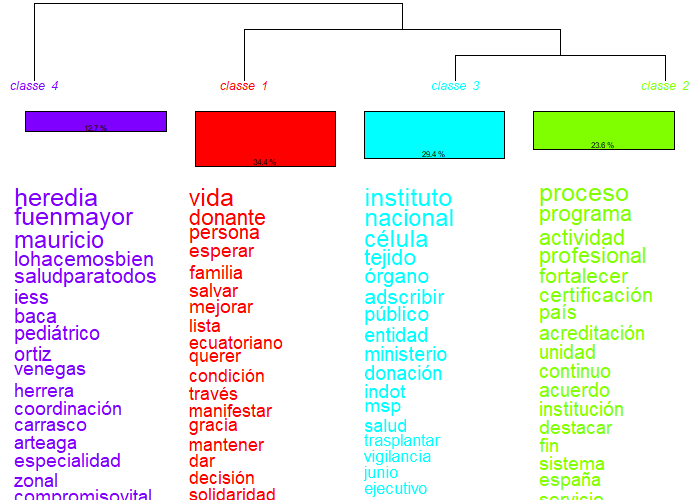
\includegraphics[width=0.9\textwidth]{figure01.png}
 \caption{Dendograma aplicado a los textos publicados por el INDOT}
 \label{fig1}
 \source{Elaboración propia, procesada desde Iramuteq}
\end{figure}

La \Cref{fig1}. Es el primer dendograma generado a partir de los textos utilizados en las publicaciones de la \emph{fanpage} de Indot. En el mismo, se pueden visualizar cuatro clases que se describen a continuación. La clase 4, de color violeta, tiene una presencia del 12,7\% en el texto analizado, la misma hace referencia a nombres y apellidos de autoridades del instituto vinculados a las actividades institucionales que el Indot cumple por sí mismo o junto con otras instancias (IESS, Hospital Baca Ortiz, etcétera). Esta clase categoriza o representa los diversos hitos alcanzados en el cumplimiento de la misión institucional y cómo estos son celebrados junto con otras instituciones, el uso de hashtags \#lohacemosbien \#saludparatodos y \#compromisovital destaca en estas publicaciones. 

La clase 2, de color verde corresponde a un 23,6\% de presencia. Esta clase pone de relevancia como el Indot ha llevado adelante iniciativas de acreditación, certificación y fortalecimiento de profesionales de la salud y unidades médicas en cuanto a la donación y el trasplante. En esa línea, el Art. 19 de la Ley Orgánica de Donación y Trasplante de órganos, Tejidos y Células \cite{indot2011}  menciona que los trasplantes de órganos, tejidos y células sólo podrán realizarse en instituciones de salud con autorización del Indot. 

Un ejemplo de posteo de esta clase corresponde a una publicación del 30 de abril del 2014, que informa sobre un proceso de actualización profesional: “[…] El Ministerio de Salud Pública, a través del […] (INDOT), desarrolla un programa de capacitación […] con el fin de fortalecer la actividad transplantología del país. […] el cual es coordinado por la Organización Nacional de Trasplantes (ONT) de España.”  

Con una incidencia de 29,4\%, se encuentra la clase 3, de color celeste, la cual muestra que las publicaciones del INDOT tienen un fuerte componente de promoción en sí misma, algo comprensible al ser una instancia relativamente joven que requiere aún de mucha más difusión y conocimiento de su labor entre los ecuatorianos \cite{dos_santos2020}. Así, boletines informativos, misión y naturaleza como entidad adscrita al Ministerio de salud son informaciones significativamente presentes en la \emph{fanpage}. 

La siguiente publicación del 27 de enero de 2014, es un ejemplo de esta clase: “[…] El Instituto Nacional de Donación y Trasplante de Órganos, Tejidos y Células […] informa que durante el 2013 se generaron 63 donantes de órganos, lo que representa un índice de 4.34 donantes por millón de habitantes (DPMH), evidenciándose un crecimiento del 16,6\% con relación al 2012, […]”. 

Finalmente, la clase 1, de color rojo, tiene la mayor incidencia (34,4\%) en el texto, la misma representa el énfasis de las publicaciones de INDOT hacia la importancia de la donación, no apenas como terapia médica sino como valor colectivo por alcanzarse en la sociedad ecuatoriana, de esta manera, la campaña “Historias que inspiran” así como varios boletines informativos demuestran la preocupación por vincular al ciudadano con la donación. Por ejemplo, un boletín del 22 de enero de 2013 agrupa todos estos elementos: “Boletín informativo: La solidaridad de los ecuatorianos mejoró la calidad de vida de 563 personas que necesitaban un trasplante en el 2012” (sic). 

En resumen, las cuatro clases muestran que las publicaciones del instituto se enfocan en los siguientes temas generales, en orden de importancia: Concientización de la población sobre la importancia de la donación y la promoción de valores, el INDOT como instancia pública que promueve y regula la donación y la terapia de trasplantes, actividades de acreditación institucional y actualización profesional alrededor de la donación y trasplante y; datos de tipo noticioso sobre hitos y labor cotidiana institucional.

La \Cref{fig2} corresponde al segundo dendograma generado a partir del texto con los comentarios que las publicaciones del INDOT han provocado en el periodo de estudio, por supuesto, al tratarse de expresiones ciudadanas, se esperaba una mayor dispersión en los temas, así, el análisis generó seis clases que se discuten a continuación de la figura.

\begin{figure}[htbp]
 \centering
 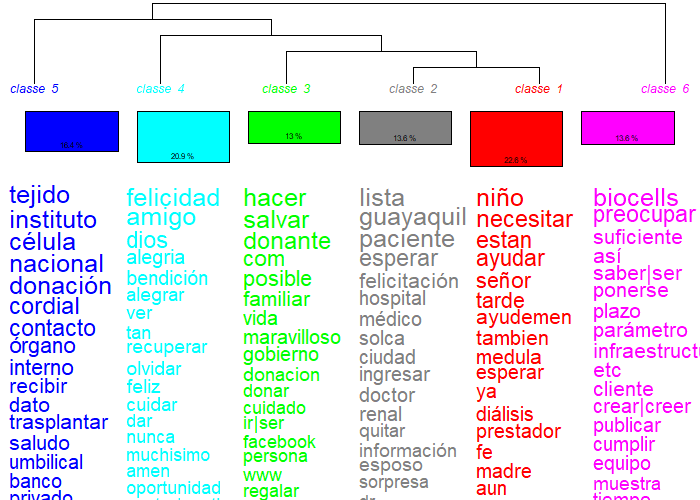
\includegraphics[width=0.9\textwidth]{figure02.png}
 \caption{Dendograma aplicado a los comentarios hechos a publicaciones del INDOT}
 \label{fig2}
 \source{Elaboración propia, procesada desde Iramuteq}
\end{figure}
 
La clase 6 de color rosado, comparte el mismo porcentaje de incidencia (13,6\%) con la clase 2 de color gris, la clase 6 representa dudas sobre un tema específico, se trata de una iniciativa privada de captación de células madre que mostró falencias señaladas por el INDOT en 2014, varios comentarios reflejan preocupación sobre muestras depositadas: “\emph{He llamado al INDOT […] BIOCELLS solo tiene un plazo de 30 días para ponerse al día con los parámetros que no ha cumplido […] Lo cierto es que como padre de familia y cliente […] estoy muy preocupado por lo que vaya a pasar con las muestras de mis hijas}.” Durante la recolección de datos no se pudo evidenciar respuesta a esta inquietud ciudadana, aún con la insistencia de la persona requirente. 

La clase 5 o clase azul con 16,4\% de incidencia, se refiere principalmente a las solicitudes de información que hace la ciudadanía al instituto incluyendo las respuestas institucionales, de allí que varias palabras se refieren a saludos formales (Cordial), solicitudes de contacto, redireccionamiento de inquietudes o preguntas sobre cuestiones específicas como el Banco Público de Sangre de Cordón Umbilical, de esta clase rescatamos un comentario ciudadano del 22 de julio de 2013: “Por favor explicar esto.... \url{ http://www.ppelverdadero.com.ec/nota-del-dia/item/alistan-banco-de-sangre-para-cordon-umbilical.html} Es decir que dos de las empresas ya dieron las muestras de células sin previa autorización de los padres.” Este comentario en particular muestra la potencialidad de la \emph{fanpage} como espacio para rendir cuentas, explicitándose que ciertos ciudadanos están ya en capacidad de no solo pedir, sino también contrastar información.

La clase 4 o celeste tiene 20,9\% de incidencia en el texto y representa las reacciones solidarias a las publicaciones del INDOT, como apoyo a posteos de  “Historias que inspiran” o para demostrar apoyo a las acciones institucionales, de allí que expresiones de alegría o felicidad son propias de la clase, como el siguiente ejemplo del 15 de diciembre de 2012, comentario a una publicación de recuperación de Nancy de 23 años, madre de familia que tuvo un trasplante renal exitoso: “Felicidades por aquellas personas que logran su objetivo, Que Dios siga bendiciendo a todos quienes hacen posible que la vida continúe., Que todos seamos donantes […]”. 

La clase 3 o verde es la de menor incidencia (13\%) e incluye expresiones como www o com ya que se acompaña de enlaces generalmente. Sin embargo, la clase tiene relevancia ya que representa ciertas interpretaciones que hace la ciudadanía sobre la donación. Así, esta clase corresponde a expresiones que muestran la existencia de sectores de la población convencidos de la importancia de esta terapia, en muchos casos las mismas personas trasplantadas que comparten su testimonio como esta publicación del 9 de marzo de 2014: “Maravilloso que hayan personas caritativas ...que regalan la vida Toda los que hacen la Unidad de Trasplante del hospital EE en conjunto con el Indot son un magnífico grupo todos los trasplantados estamos agradecidos con dios y ellos no desmayen que todavía hay personas que necesitamos de ustedes que dios los bendiga por siempre” (sic).

La clase 2 de color gris, representa a los comentarios sobre el entorno de los pacientes, tanto lo familiar, como el contexto profesional incluyendo médicos e instituciones, el vínculo que la lista de espera de trasplante crea entre las personas y las dudas vinculadas con los requerimientos para ser donante o receptor, esto último en clave de ayuda. El siguiente comentario del 8 de junio de 2015, ejemplifica la clase 2: “[…] Buenas Tardes ..Soy una Madre de un Niño con Cáncer .Leucemia […] EN SOLCA VENGO YA CON EL TRATANDOLO TRES AÑOS ..A COJIDO quimio terapias .[…] El Medel tratante de mi hijo .me dice que esta para un trasplante de médula ...[…]No quiero que […] vuelva recaer .por falta de una médula ..ayúdenme .mi hijo tiene todas las ganas de vivir ...”.

Resulta importante mencionar que tanto la ciudadanía, como los pacientes y sus familiares, no tienen claro los procesos que deben seguir para ingresar a la lista de espera, y en ciertos casos tampoco conocen el proceso para ser donante, vale la pena reflexionar sobre la necesidad de impactar y socializar estos procesos en la ciudadanía, más aún cuando existe un público que se acerca a la institución.

La clase 1 de color rojo agrupa también pedidos de ayuda o apoyo para trasplante, pero escritos en primera persona, es decir, salen de los propios ciudadanos en necesidad de órganos. Vale decir que la lista de espera de trasplante es demasiado larga, de allí que esta y otras investigaciones buscan impulsar una mayor disponibilidad de órganos para estas personas. Una publicación del 2 de octubre de 2020 pide información, al tiempo que se refiere una necesidad familiar: “Como puedo inscribirme para ser donante […] cuanto le ruego a mi Dios que ayude a mi padre y pueda volver a ver la luz algún día […] ayúdenme a que mi padre tengas sus corneas él también está en lista de espera”; de este comentario vale notar que la persona desconoce que en cumplimiento de la Ley orgánica de donación y trasplante de órganos y tejidos todo ecuatoriano es donante en principio.

Finalmente, vale recordar que muchas de las publicaciones -no solo en Facebook, sino en todo tipo de plataformas \cite{cisco2016}- son principalmente visuales, si bien este tipo de discursos requieren otros análisis que salen de los propósitos de esta investigación, se realizó un esfuerzo adicional para capturarlos de cierta forma considerando que 724 (90,4\%) de las publicaciones durante el periodo de estudio estaban acompañadas de imágenes o similares. Así, la matriz de datos incluyó una columna donde se describía lo visto o se capturó directamente el texto dentro de la imagen -diferente del texto del posteo- esa columna fue también analizada con Reinert, como se puede observar más adelante. 

\begin{figure}[htbp]
 \centering
 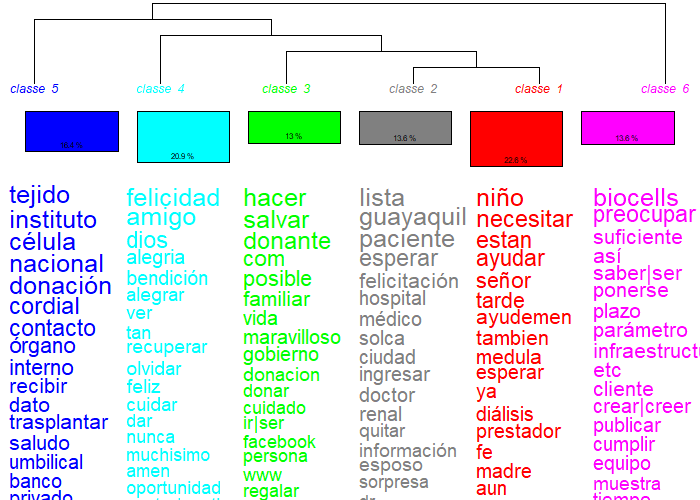
\includegraphics[width=0.9\textwidth]{figure02.png}
 \caption{Dendograma de las descripciones de imágenes y videos publicados por INDOT}
 \label{fig3}
 \source{Propia, obtenida desde Iramuteq}
\end{figure}

El análisis de texto correspondiente a imágenes o videos se divide en cinco clases, la clase 5 con 21,4\% de representatividad muestra principalmente cómo la concienciación de la población alrededor de la donación, se apoyó en varios casos en infografías, colocando una idea central apuntalada en datos estadísticos (casos, número, personas, etcétera) presentados como esquemas gráficos. Esta estrategia se usó también en la presentación de resultados, e informes sobre la pandemia de la Covid-19, aunque la mayoría de estas publicaciones fueron reposteos del Ministerio de Salud.

La clase 1, de color rojo, también con 21,4\% muestra como el quehacer cotidiano del Indot se informa a la población con fotografías de certificaciones en hospitales, inicios y cierres de capacitaciones, inauguraciones, personal e infraestructura del instituto. Por su lado, la clase 4 (18,2\%) representa las imágenes vinculadas con las historias de los pacientes trasplantados, con énfasis en el impacto que la donación tiene en sus vidas, estas imágenes forman parte de la campaña “Ecuador dona vida”, que invita al público a mantener su condición de donante. Además, esta clase también resalta las jornadas médicas a las cuales asisten los profesionales de la salud.

En cuanto a la clase 3, (18,2\%) representa los videos o imágenes utilizados para convocatorias a contratación y concursos de méritos, principalmente para médicos (publicaciones originales del Ministerio de Salud) o invitaciones a colaborar como es el caso de donantes voluntarios de sangre; destacan también imágenes con saludos y deseos por año nuevo, así como imágenes que presentan información sobre la gestión institucional, por ejemplo, una imagen del 07 de septiembre del 2019 hace referencia a un informe que destaca que en 13 años se han realizado 5.741 trasplantes en el país. Finalmente, la clase 2 muestra como un importante componente de las imágenes y videos se enfocan en las autoridades, tanto del INDOT como de instituciones vinculadas, de allí que existan referencias a apellidos correspondientes a distintos representantes.

En resumen, la \Cref{fig3} muestra cómo las publicaciones de la página hacen uso de imágenes en dos contextos: el primero en el que la clase 5 detalla información estrechamente relacionada a la pandemia y engloba publicaciones que pertenecen a otra institución pública (Ministerio de Salud), y el segundo que agrupa el resto de clases, con temas, en su mayoría, originales del INDOT, como casos de éxito en trasplantes, capacitaciones, campañas para promover la donación, convocatorias y menciones de autoridades propias y de sus instituciones vinculadas.

\section{Discusión}\label{sec-discusion}

Es importante señalar que las redes sociales han comenzado a desempeñar un papel importante en la salud pública, especialmente en campañas de difusión, aplicadas a áreas tan diversas como la prevención del suicidio, obesidad infantil y actitud hacia la vacunación \cite{luxton2012, salathe2011, vandewater2011}. Desde su lanzamiento en febrero de 2004, Facebook ha demostrado ser muy eficaz en la creación de oportunidades para que un mensaje en particular llegue a una audiencia masiva. Más recientemente, estas oportunidades se han extendido a la donación de órganos, un área que podría beneficiarse de la atención de la red social \cite{cameronetal2013, greenemeier2012}.

De hecho, con la creciente demanda de órganos para trasplantes en el mundo, Facebook ya se ha convertido en un canal popular para las personas que solicitan riñones, hígados y otros órganos que pueden salvar vidas \cite{cameron2015, cameronetal2013}. En el año 2012, la red social comenzó a ofrecer a sus miembros de Estados Unidos la posibilidad de identificarse como donantes de órganos y de ubicar los registros estatales de donación de órganos si querían convertirse en donantes \cite{greenemeier2012}.

Esa potencialidad podría ser muy útil en el Ecuador, por varios factores, el primero de ellos que la normativa vigente desde 2012 hace de todo ecuatoriano un donante a menos que señale lo contrario. A partir del registro y ejecución de dicha ley el número de donantes registrados ha ido en aumento, siendo así que, el año 2019 la tasa de donantes por millón de habitantes (PMH) aumentó a 7,75 con respecto al año 2012 que la tasa de donantes PMH era de 3,48 \cite{indot2011}. Se observa una visibilidad cautiva y voluntad de ser donante de órganos y de recibir más información sobre este tema en ciertos sectores de la población y adicionalmente se están juntando factores psicosociales y reflexiones académicas que aportan a tomar posiciones respecto a la donación \cite{dos_santos2020, dos_santos2019}. 

De todas formas, vale decir que en la práctica aún no se han conseguido los resultados deseados alrededor de la donación, que tiene varios desafíos, incluyendo elementos culturales que no cambian por decreto, por lo cual es preciso establecer formas de reposicionar este tema en el imaginario colectivo para conducir la acción social. Así, analizar cómo la difusión del registro para la donación de órganos puede apoyarse en plataformas de redes sociales como Facebook. La cual representa una oportunidad para aprender cómo conductas y decisiones relacionadas con la salud se pueden transmitir y profundizar dialógicamente, conocimiento útil para diseñar intervenciones futuras y elevar las tasas de donación de órganos, actualmente en índices muy bajos.

Entre las características halladas en esta investigación, respecto a los actuales niveles de interacción de la \emph{fanpage} del INDOT, se encontró que la página tiene niveles aceptables de visibilidad, compartición y evaluación, trabaja con publicaciones principalmente originales y se evidencia un apoyo institucional a la difusión por redes. Sin embargo, los índices de interacción aún pueden mejorarse, enfocándose en el uso de narrativas visuales, estadísticas y narración de historias personales. Justamente, varias investigaciones realizadas en cuanto a las características que deben tener las publicaciones de ONG en Facebook detallan que el humor, la emoción y los componentes afectivos son elementos importantes para la viralización de los posteos \cite{arroyo-almaraz2018}.


\printbibliography\label{sec-bib}

%\begin{contributors}{sec-contributors}
%\item \textbf{Gabriel Francisco Cevallos Martínez}:  Conceptualization, Methodology, Formal analysis y Writing (draft) e Writing (editing);
%\item \textbf{Jonathan Bladimir Zhiminaicela Cabrera}: Resources and Formal Analysis;
%\item \textbf{María Fernanda Fernández Gonzales}: Resources and Formal Analysis;
%\item \textbf{Sueny Paloma Lima dos Santos}: Conceptualization, Writing (review e editing).
%\end{contributors}

%full list: conceptualization,datacuration,formalanalysis,funding,investigation,methodology,projadm,resources,software,supervision,validation,visualization,writing,review
\begin{contributors}[sec-contributors]
\authorcontribution{Gabriel Francisco Cevallos Martínez}[conceptualization,methodology,formalanalysis,writing] %\authorcontribution{conceptualization,methodology,formalanalysis,writing}
\authorcontribution{Jonathan Bladimir Zhiminaicela Cabrera}[resources,formalanalysis] %\authorcontribution{resources,formalanalysis}
\authorcontribution{María Fernanda Fernández Gonzales}[resources,formalanalysis]
\authorcontribution{Sueny Paloma Lima dos Santos}[conceptualization,review]
\end{contributors}


\end{document}
